%% ----------------------------------------------------------------
%% Thesis.tex
%% ---------------------------------------------------------------- 
\documentclass[openany,12pt]{ecsthesis}      % Use the Thesis Style
% Location of your graphics files
\usepackage[numbers]{natbib}            % Use Natbib style for the refs.
\hypersetup{colorlinks=false}   % Set to false for black/white printing
\input{Definitions}            % Include your abbreviations
\usepackage{listings}
  \usepackage{color}
  \definecolor{lightgray}{rgb}{.9,.9,.9}
  \definecolor{darkgray}{rgb}{.4,.4,.4}
  \definecolor{purple}{rgb}{0.65, 0.12, 0.82}
  \usepackage{graphicx}
  \usepackage{float}
  \usepackage{listings, xcolor}
  \definecolor{verylightgray}{rgb}{.97,.97,.97}
  \lstdefinelanguage{Solidity}{
    keywords=[1]{anonymous, assembly, assert, balance, break, call, callcode, case, catch, class, constant, continue, contract, debugger, default, delegatecall, delete, do, else, emit, event, export, external, false, finally, for, function, gas, if, implements, import, in, indexed, instanceof, interface, internal, is, length, library, log0, log1, log2, log3, log4, memory, modifier, new, payable, pragma, private, protected, public, pure, push, require, return, returns, revert, selfdestruct, send, storage, struct, suicide, super, switch, then, this, throw, transfer, true, try, typeof, using, value, view, while, with, addmod, ecrecover, keccak256, mulmod, ripemd160, sha256, sha3}, % generic keywords including crypto operations
    keywordstyle=[1]\color{blue}\bfseries,
    keywords=[2]{address, bool, byte, bytes, bytes1, bytes2, bytes3, bytes4, bytes5, bytes6, bytes7, bytes8, bytes9, bytes10, bytes11, bytes12, bytes13, bytes14, bytes15, bytes16, bytes17, bytes18, bytes19, bytes20, bytes21, bytes22, bytes23, bytes24, bytes25, bytes26, bytes27, bytes28, bytes29, bytes30, bytes31, bytes32, enum, int, int8, int16, int24, int32, int40, int48, int56, int64, int72, int80, int88, int96, int104, int112, int120, int128, int136, int144, int152, int160, int168, int176, int184, int192, int200, int208, int216, int224, int232, int240, int248, int256, mapping, string, uint, uint8, uint16, uint24, uint32, uint40, uint48, uint56, uint64, uint72, uint80, uint88, uint96, uint104, uint112, uint120, uint128, uint136, uint144, uint152, uint160, uint168, uint176, uint184, uint192, uint200, uint208, uint216, uint224, uint232, uint240, uint248, uint256, var, void, ether, finney, szabo, wei, days, hours, minutes, seconds, weeks, years},	% types; money and time units
    keywordstyle=[2]\color{teal}\bfseries,
    keywords=[3]{block, blockhash, coinbase, difficulty, gaslimit, number, timestamp, msg, data, gas, sender, sig, value, now, tx, gasprice, origin},	% environment variables
    keywordstyle=[3]\color{violet}\bfseries,
    identifierstyle=\color{black},
    sensitive=false,
    comment=[l]{//},
    morecomment=[s]{/*}{*/},
    commentstyle=\color{gray}\ttfamily,
    stringstyle=\color{red}\ttfamily,
    morestring=[b]',
    morestring=[b]"
  }
  
  \lstset{
    language=Solidity,
    backgroundcolor=\color{verylightgray},
    extendedchars=true,
    basicstyle=\footnotesize\ttfamily,
    showstringspaces=false,
    showspaces=false,
    numbers=left,
    numberstyle=\footnotesize,
    numbersep=9pt,
    tabsize=2,
    breaklines=true,
    showtabs=false,
    captionpos=b
  }
%% ----------------------------------------------------------------
\begin{document}
\frontmatter
\title      {Distributed ledgers application in Science: \\
Smart Papers on the Ethereum}
\authors    {\texorpdfstring
             {\href{mailto:yx5u17@soton.ac.uk}{Yixuan Xu}}
             {Yixuan Xu}
            }

\supervisors{\texorpdfstring
             {\href{e.simperl@soton.ac.uk}{Professor Elena Simperl}}
             {Professor Elena Simperl}
            }

\examiners  {\texorpdfstring
             {\href{mailto:gvm@ecs.soton.ac.uk}{Dr Geoff Merrett
             }}
             {Dr Geoff Merrett}
            }

\addresses  {\deptname\\\univname}
\date       {\today}
			
\subject    {}
\keywords   {}
\maketitle
\begin{abstract}
This work is all about \dots
\end{abstract}
\tableofcontents
\listoffigures
\listoftables
%\lstlistoflistings
%\dedicatory{To \dots}
\mainmatter
%% ----------------------------------------------------------------
\chapter{Introduction}
\section{Project aim}
\paragraph{}Digitization and Web technologies are now changing the way of publishing and disseminating the knowledge.
It becomes more convenient and less expensive for people to access the knowledge. 
The knowledge creation process is more dynamic right now. 
Text/graphics/rich media can be changed quickly and easily while at the same time being available to all the audiences.
However, most of current methods of academic publication are static, that means, they cannot be revised over time\cite{heller2014dynamic}. 
Web technologies actually have the power to make it more dynamic but is currently underused. On the other hands, journals, publishers and funders fully control
the entire process of academic publishing. The view of authors who should also participate in the publishing process tends to be underrepresented. 
Despite that fact that the current academic publishing system is advance and productive, 
authors still want a more open and decentralize publishing process \cite{d2018authors}.
\paragraph{}In the past, the scholarly books were keeping improving and updating for the centuries by releasing the new editions. 
Mistakes would be corrected, new result would be added and feedbacks would be used for improvement. 
Revising books allowed author to keep track with novel development \cite{heller2014dynamic}. 
Many handbooks and schoolbooks have been revised over and over again, resulting massive amount of quality publications.
In the contrast to books, academic paper were a kind of snapshot of certain scientific knowledge. 
Most of them were just published once. If there is a new finding, usually a new articles need to be published. 
But this kind of process are currently under debate and development \cite{heller2014dynamic}. 
The number of authors who want a more open process in scientific publishing is increasing rapidly. 
When it comes to the traditional of academic publishing, 
publishers play an important role of filtering good research, rejecting papers 
without sufficient conclusions. 
They make their decisions based on the peer-review process which is fully controlled by themselves. 
Since this kind of peer-review process usually will take a significant amount of time and is one of the
main reason of delaying publications, researcher came up with a new idea of doing publishing. A initial version
will be firstly released, then it could be updated after receiving the feedbacks from pre-peer-review. 
All the version will be always available and the changes made in the pre-peer-review process will also be stored after the publishing of final version.
The model allows the tracking of the development of academic papers. 
This improvements make the process of publishing process more dynamic and flexible.
But, there are some vital problems that have been discussed under such models 
which is the mechanism to manage the interactions between authors and contributor in a trust way \cite{Khoe:1994:CML:2288694.2294265}.
How can authors make agreements with each other about which version should be available ?
How can authors determine their contributions to the papers in a unprejudiced way ? On the other hand,
the contributions of reviewers is ignored in this model.
\paragraph{}In last few years, Distributed Ledger Technology have attracted public attentions as 
the most advanced tool that can provide a decentralized solutions to manage the interaction 
between people that may not trust each other. 
It also could guarantee the security and consistence without the need for admin. 
The special tools which could achieve such functionality is called Smart Contract. For the questions about the publishing model,
Smart contract could be programed to help authors to making decision in a decentralized way. The aim of this project is trying to provide a prototype of decentralize application 
to help authors to manage their publish and their attribution agreements in a dynamic and trusted way. 
The application itself will use the blockchain technology \cite{buterin2013ethereum}, so nobody can fully control the whole process.
It could be more reliable than the current publishing system. 
The implementation will be evaluated by the cost of using such system. 
A detailed cost analysis and data visualization will also be presented.  
\section{Outline}
\paragraph{}In Section 2, firstly it will present some modern publishing systems based on the blockchain.  
Then a general background of blockchain will be presented. After that, 
a more specific description about the smart contract on Ethereum would be shown for the following part
\paragraph{}In Section 3, it would give detailed design of the application. 
By comparing the blockchain technology with the current Web technology, 
It should gives more clear explanation why blockchain is preferred for this project
\paragraph{}In Section 4, it will focus on the Implementation. 
All the important implementation details will be described here
\paragraph{}Section 5 demonstrate the cost of using the decentralize application. 
The analysis consists of the visualization and specific code review.
\paragraph{}Section 6 will discuss the advantage and disadvantage of the current implementation.
Potential improvement would also be covered in this section.
\paragraph{}Section 7 will give a summary about the project and conclusion.
\chapter{Background Research}
\section{Modern publishing models example}
\paragraph{}Because of the development of web technologies, 
several models have been provided based on the modern web technologies to improve the process of the academic publish, 
making authors manage and produce their works more easier. 
DEIP \cite{DEIP} is a platform that aimed at effective and 
fair distribution of resource allocated to scientific and research activities.
It proposed a community-driven models that encourage the open knowledge without restriction.
The users of this platform could be both author and reviewers and have free access to all the publications. 
All the records of reviews will be recorded and reviewers will be awarded by the decentralized protocol.
Scienceroot \cite{science} is another blockchain-based publishing platform, 
it tries to creating a scientific publishing model which will reward and sustain researchers instead of maximizing the publishers' profits 
by using a fully decentralized storage platform called IPFS \cite{benet2014ipfs}. 
The Pluto \cite{Pluto} is also a platform that is trying to help researchers to get funding in a decentralized ways. 
It also wants to establish a more proper evaluation index for the academic publications. 
The ideas of these kinds of platforms are really aggressive but inspiring. 
They are trying to give the power back to authors and reviewers and to make the knowledge more open and accessible to everyone.
It could be found that modern publishing system requires more transparent review process and more trustable collaborations between authors.
The current Blockchain technologis have huge potential in aspect of creating decentralized application. So it could be found that all of above platform are 
using the Ethereum \cite{buterin2013ethereum} as their core framework. 
\section{Blockchain}
\subsection{Technology}
On its most basic level, 
the blockchain is a new kind of information technology 
which is the combination of encryption methods with distributed computing.
Satoshi Nakamoto \cite{nakamoto2008bitcoin} combine them to make new ways to create a model 
where a network of computers collaborate to maintain a shared and secure database. 
This database consists of a string of blocks each one a record of data 
that has been encrypted and given a unique identifier called a hash.
Mining computers on the network validate transactions, 
add them to the block they are trying to build, 
and then broadcast the completed block to other nodes 
so that all have a copy of the database. 
Because there is no centralized server to validate the transaction to the database,
the blockchain depends upon a distributed consensus algorithm. 
In order to make an entry on to the blockchain database, 
all the computers have to agree about its state 
so that no one computer can make an alteration without the consensus of all others.
Once completed, a block goes into the blockchain as a permanent record. Each time a block get completed, a new one will be created.
Countless number of block connect to each other, like links in a chain. The kind of data structure makes the transactions immutable.
Every block contains hash value that is dependent on the hash of the previous block, 
if one is changed than all the other blocks linked to it going forward will be altered.
This works to make the data entered tamper-proof. 
This model is the working mechanism of the first generation blockchain which is known as Bitcoin.
Its functionalities are mainly focused on the small data storage, which is the history of transactions.
Blockchain are trying to create a secured, trusted, 
shared database and they do this through encryption and hashing,
proof of work and network consensus. The hashing and linking of blocks 
makes it difficult to go back and change a previous block once entered. 
And the proof of work system intentionally makes it computationally more difficult to alter the database,
thus making it extremely difficult to change all the blocks. It leads to a distributed consensus mechanism so that even if someone did it,
it is almost impossible to convince others to accept as the valid record. The bitcoin blockchain is a very good proof of the stability of such system.
It now secure hundreds of billions of dollars using this method without the network having been hacked. 
What this technology enables is a database that is secure with automatic trust 
which is powered by open source community and encryption.
It is tamper proof, once information is put into the database it can not be altered. 
It is a shared database as many people would have a up-to-date copy so that all have a single source of truth.
Likewise, it is transparent, all the transactions and alteration made to the blockchain is visible to everyone.
\subsection{Ethereum}
With in a few years,
the second generation of blockchain emerged design as a network on which developers could build applications. 
It is going to be more like a distributed virtual computer than just database.
This was made technically possible by the development of the Ethereum platform. 
Ethereum is an open-source, public, blockchain-based distributed computing platform featuring smart contract functionality.
It provides a decentralize Turing-complete virtual machine, which can execute computer programs using a global network of nodes.
Ethereum was initial described in a white paper by Vitalik Buterin \cite{buterin2013ethereum}. 
The system has been very successful attracting a large and dedicated community of developers, supports and enterprises.
The important contribution of Ethereum as the second generation of blockchain is that 
it worked to extend the capacity of the technology from primary
being a database to becoming more a general platform for running decentralized application and smart contracts.
It provides developers with a powerful but simple turing-complete language called Solidity that used for build smart contracts.
As of 2018 Ethereum is largest and most popular platform for building distributed application. 
It has been a major step forward to become a global distributed computer, 
a massive globally distributed cloud computing platform upon which we can run any application at scale and speed,
with the assurance that it has the security, resilience and trustworthiness of today's blockchain.
\paragraph{}
By reviewing the blockchain technology, 
it is easy to find out that Ethereum is really powerful to
help authors to make agreements and set their outcomes in stone so that they cannot be later repudiated.
In \cite{Khoe:1994:CML:2288694.2294265}, 
the Smart Paper model is proposed to provide a collaborative platform 
that preserves a single version of the truth through the collaborative process. 
Authors will use the smart contract to publish their works and collaborate with others.
Once decision is made, smart contract will guarantee the result of decision won't be change by anyone.
All the versions and meta data about contributions will be safely stored on the Ethereum.
\chapter{Design}
For a information system, the state flow and data structure are the two key point.
The state flow is related to the service logic. It concerns how to operator data, how data changes. 
The application interface and the implementation of interact should be built based on those information
For a traditional publish model, it could be described as \ref{model}.
\begin{figure}[H]
  \centering
  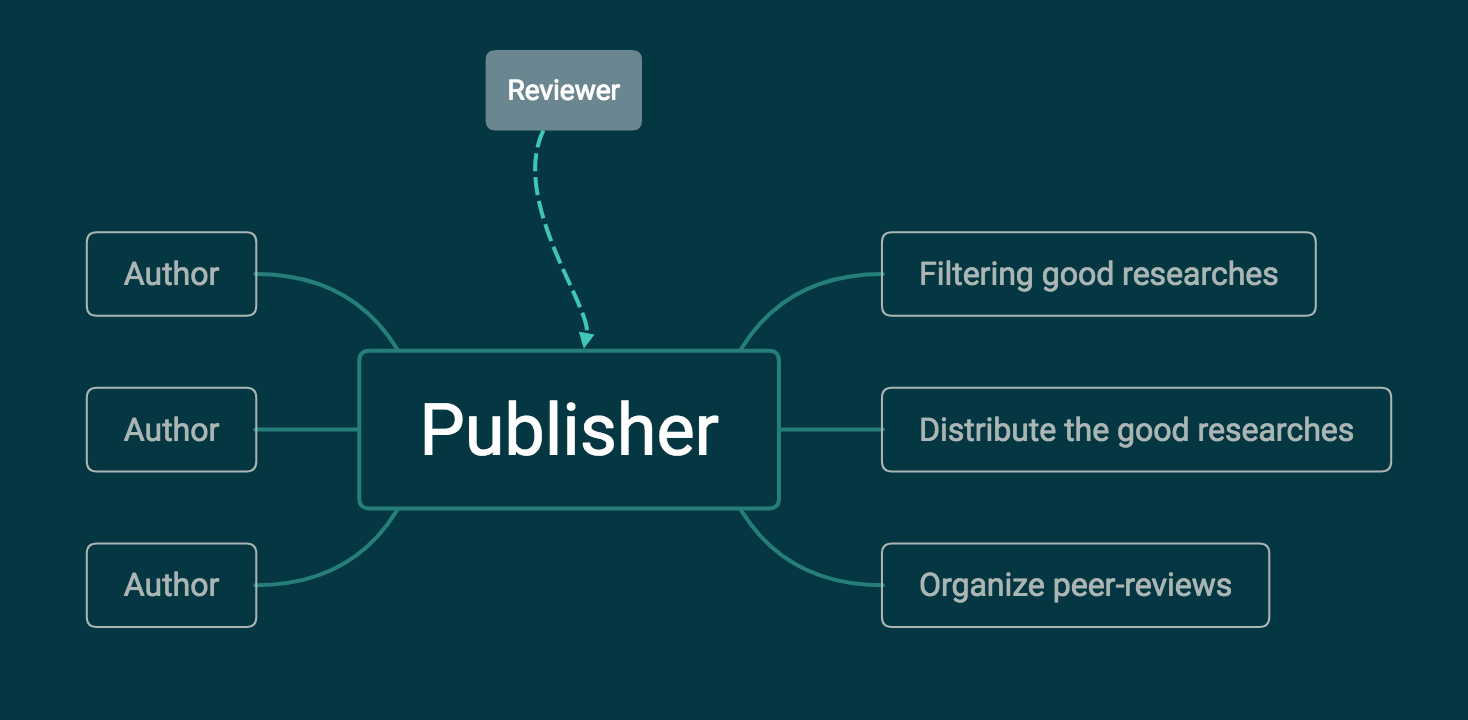
\includegraphics[width=0.9\textwidth]{traditionModel.png}
  \caption{Traditional publish model}
  \label{model}
\end{figure}
In this model, publishes takes all the responsibilities of filtering the good researches, 
rejecting papers with methods that are insufficient to draw the stated conclusion and the distributing widely\cite{heller2014dynamic}. 
The whole system is too centralized. 
On the other hand, the process of producing paper is not transparent to the public. It is hard for authors to determine their contributions for the paper.
The peer-review process is also not transparent enough. There should be a channel for authors and publishers to exchange those vital information.
\section{Requirements}
The first step of software developing is to identify the requirements from the specification,
then finding the correspond user cases.
The aim of this project is to provide a prototype of decentralize application 
to help authors to manage their publish and their attribution agreements.
Based on this, we could have these simple user cases:
\begin{itemize}
  \item Researchers should have their identities based on addresses of their Ethereum accounts
  \item Researchers should be able to use smart contract to publish a research artifacts, which will be represented by the hash of files
  \item Researchers should be able approve the contracts that belongs to themselves after verifying their local files with the online files with respect to a specific version
  \item The paper contracts should contains the description, metadata and version list of the research artifacts.
  \item The contents of papers could be update with the agreements of all authors. 
  \item New researchers could be added to an ongoing paper with the agreements of all the previous researchers.
  \item The application should be open sourced and decentralized. Anyone could deploy their own instances.
  \item The review process could be community-driven and powered by publisher.
\end{itemize}
\begin{figure}[H]
  \centering
  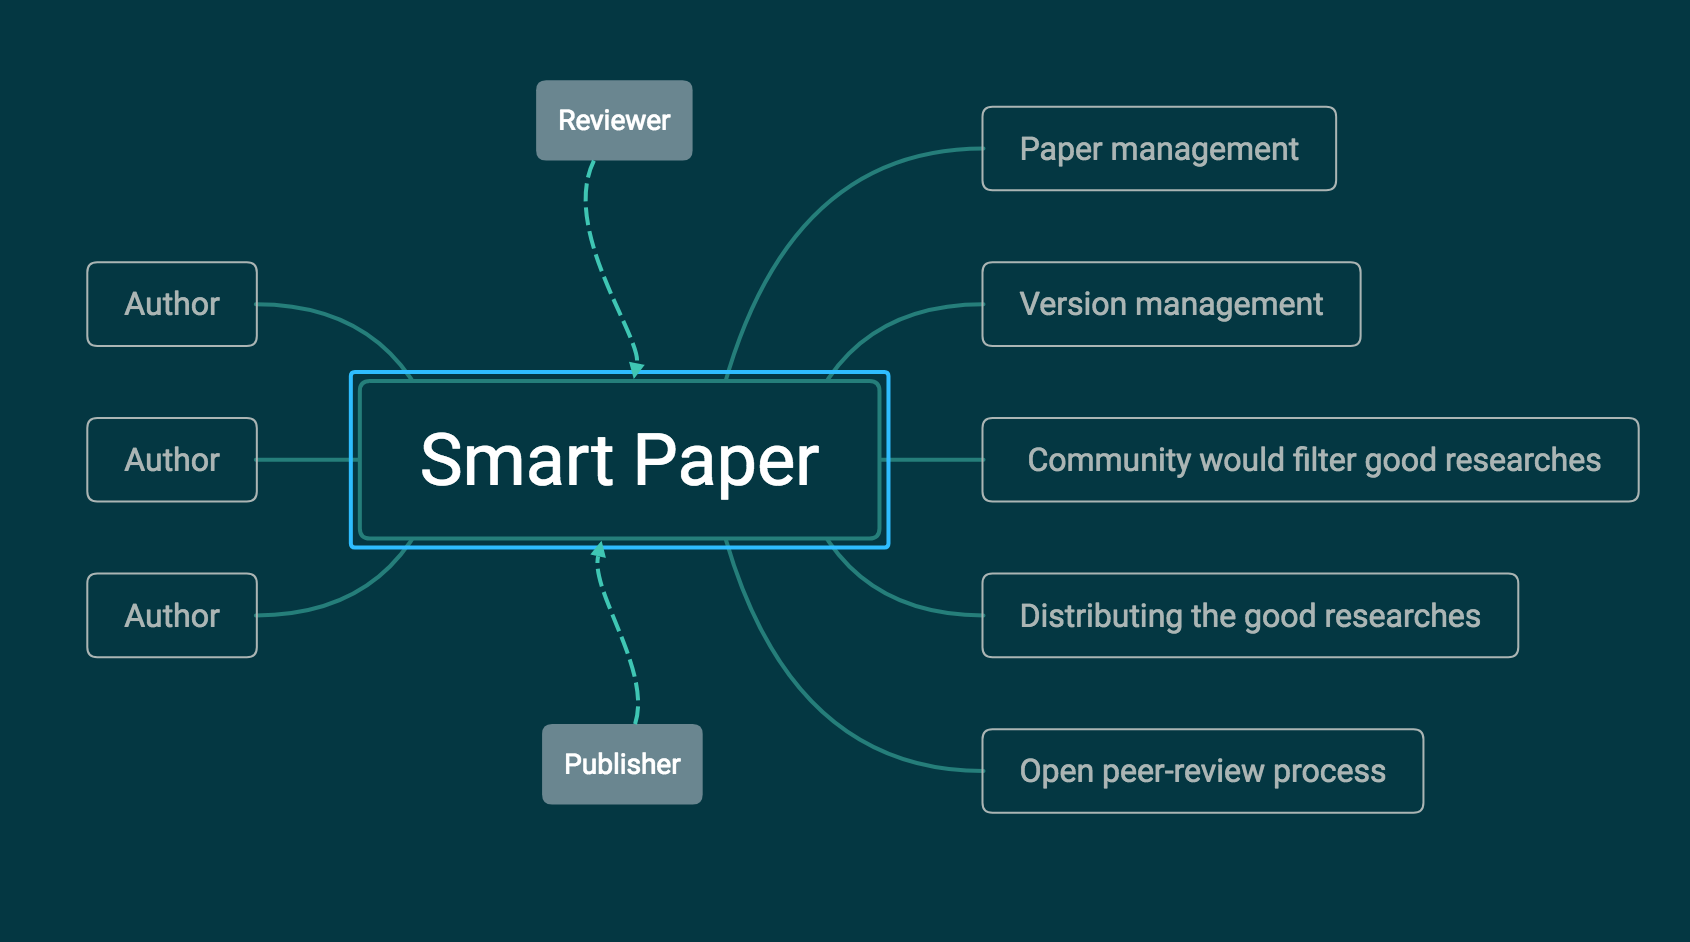
\includegraphics[width=0.9\textwidth]{smartPaperModel.png}
  \caption{Smart paper publish model}
  \label{smartPaper}
\end{figure}
The smart paper be design based these requirements. 
Based on the power of smart paper, we could have a new mechanism described as figure \ref{smartPaper}. 
In this model, the whole process of publishing would not be controlled by any individuals or organizations.
Authors could use the smart paper to do their publishing which will keep the full records of producing process. 
publisher could use smart paper to organize open peer-review. 
The smart paper will be a powerful but user-friendly tool for both authors and publishers.
Their contribution will be recorded permanently on the Ethereum. 
The smart paper consists of smart contracts which is used to implement those functionalities. 
\section{Data structure}
The fundamental data unit for the smart contract used in these project is paper, 
which could be created and managed by authors and be reviewed by reviewers.
the paper has it own basic properties such as description, metadata, hash of files and the list of authors.
Here are the properties that should be included in the paper contract:
\begin{itemize}
  \item \textbf{Description} the description of these paper, which help reviewer to understand the area of the paper.
  \item \textbf{Metadata} the metadata of these paper, which contains the contributions, comments and all the other important metadata of the paper.
  \item \textbf{latestMd5} the hash of files, which is the latest version.
  \item \textbf{versionNumber} the number of latest version, which will shows the latest published version to the public.
  \item \textbf{authorList} the list of Authors, which is the users who could control this contract
  \item \textbf{versionList} the list of versions, which contains of all the version in these contract.
  \item \textbf{isAuthor} a mapping of address to boolean value, which indicate that if the user is the author of paper.
\end{itemize}
The version of paper has complicated structure so we have to use a special keywords called 'struct' to construct it. 
This keyword works like 'struct' in C programing language.
For version, there are some properties:
\begin{itemize}
  \item \textbf{versionNumber} the unique Id for the current version.
  \item \textbf{md5} the hash of current version.
  \item \textbf{isPublished} the status of current version.
  \item \textbf{isSigned} the mapping of address to boolean, which indicate if the author is agreed this version
  \item \textbf{voterCount} the number of how many authors is agreed with this version, if the number is equal to number of authors, the state of version will be changed
\end{itemize}
These is the key design of the data structure of the project. The rest of design of the other contracts could be found at the source code.
\section{Smart Contract}
Three kinds of contracts, 
which are RBAC(Role based access control), smartPaper and smartPaperList, 
will be used in this project.
\begin{figure}[H]
  \centering
  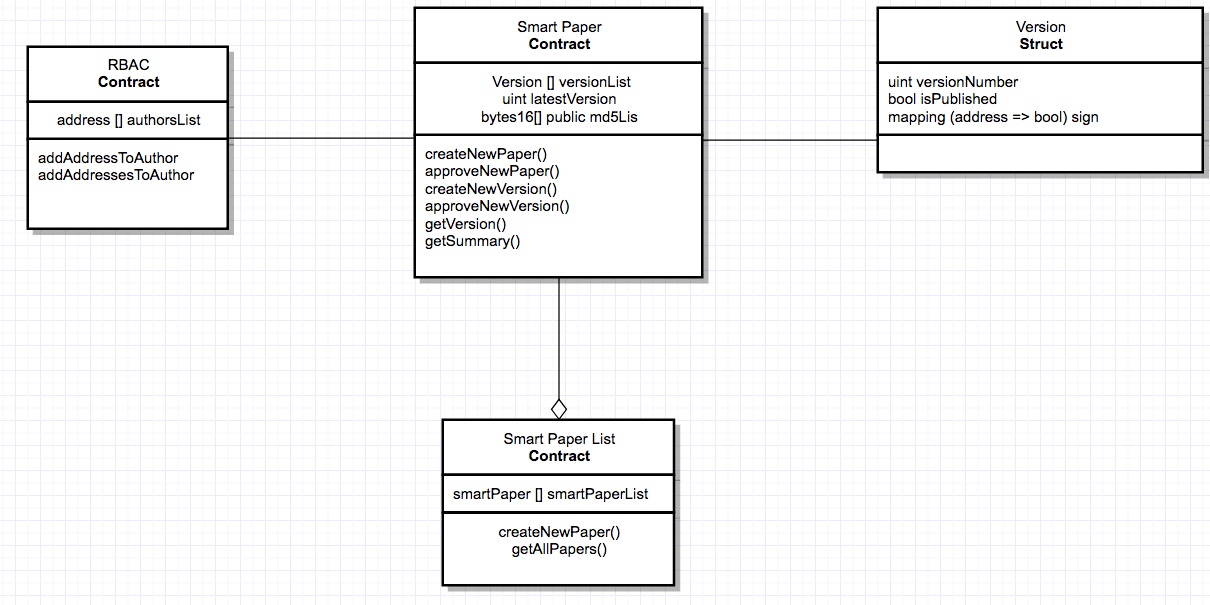
\includegraphics[width=1.0\textwidth]{uml.png}
  \caption{Smart Paper Design}
  \label{uml} 
\end{figure}
The initial design in design in \cite{Khoe:1994:CML:2288694.2294265} consider the single version of paper as a standalone contract.
However, it will increase the cost of smart paper. The current design is more cheaper by making the single version just a special data structure.
RBAC is a special contracts used for access managements. It maintain a hash table of the address of authors. 
Every time authors want to publish or approve a new version, 
RBAC will check the if authors belongs to this paper. 
Smart paper contains all the core functionalities, 
in the prototype application the hash of file will be stored instead of real file. The description and metadata will also stored in the contract.
Author can use the smart paper contract to publish new versions, then others authors need to approve the new version.
Once the new version is confirmed, 
it would be public available to the reviewers.  
The smart paper list contract is used to control all the smart paper and create new smart papers. 
It is the entry point of application.
\section{The Smart Paper workflow in Ethereum}
To begin with, a description of paper, metadata of paper, an array of addresses of authors and the file is submitted by a writer. 
The smart paper list will take those information and create a new smart paper contract which contains all the information. 
Then all the authors need to use the new smart paper contract to approve the initial version. Once a new version is finished, 
follow the same step, 
writer need to use smart paper contract to release a new version by providing the new description, metadata and file.
Then all the authors also need to approve the new version to make it public.
The smart paper workflow involves multiple working versions with dynamic collaborators. 
Version can become published and made available for annotating.
The smart paper list contract will keep the records of all the smart paper create by itself. 
User can access addresses of all the smart papers through this contract and check specific information of a paper by a specific address.
\chapter{Implementation}
\section{New web service}
\begin{figure}[H]
  \centering
  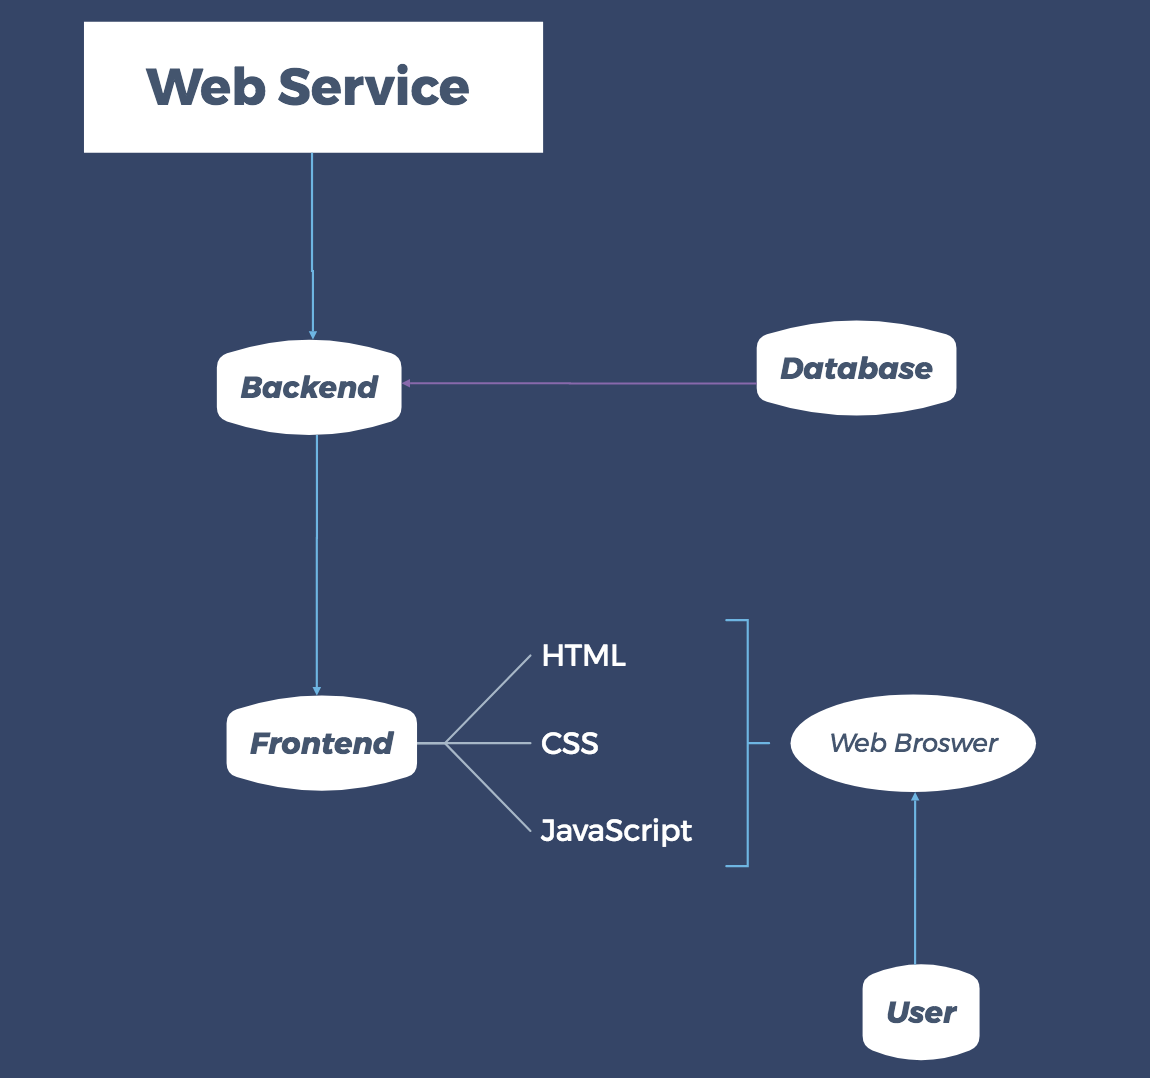
\includegraphics[width=0.8\textwidth]{triditionalWebService.png}
  \caption{Traditional Web Service}
  \label{service} 
\end{figure}
What the Ethereum platform really provides with the developers is a new kind of fundamental infrastructure for the current web service.
The traditional web service, which could be described as \ref{service}, is a too centralized system.
The backend and database are fully controlled by cloud service providers. If developers want to store their data safely, 
they have to chose those big companies such as Google and Amazon, which is expensive. 
Otherwise, they may suffer from the data loss. 
Cloud service providers have the admin accounts that could access all of the data even modify them without any permission.
The blockchain technologies could change this situation.
\begin{figure}[H]
  \centering
  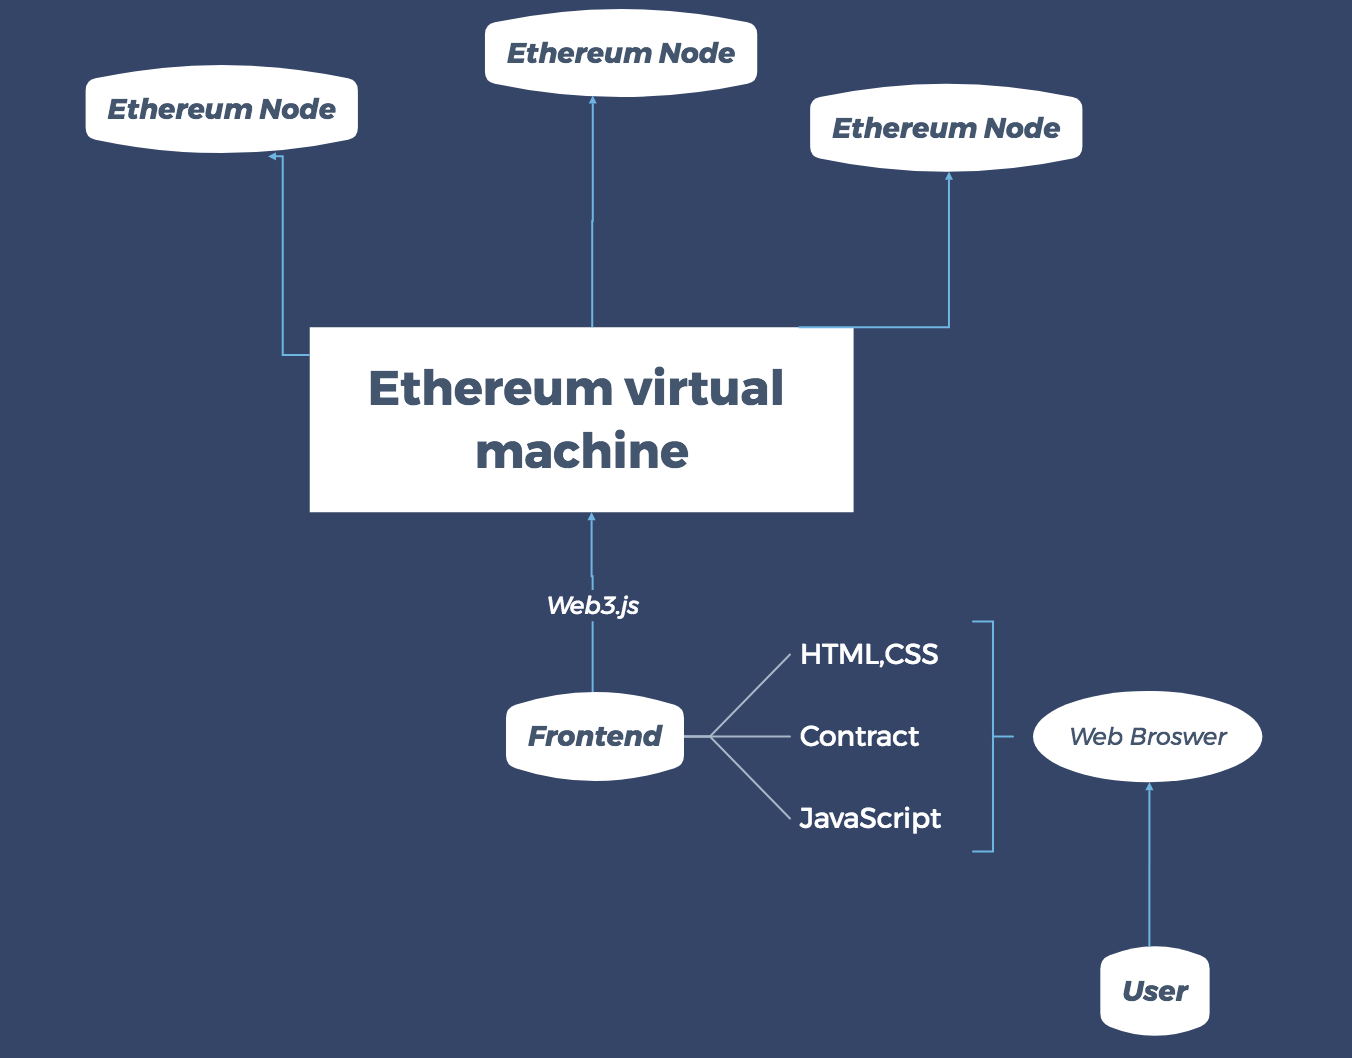
\includegraphics[width=0.8\textwidth]{EthereumWeb.png}
  \caption{Decentralized web service}
  \label{newservice} 
\end{figure}
\ref{newservice} illustrates the new design of decentralized application. Developers will program the service into the contract. 
For the project, all the functionalities of requirements will be coded into three contracts. The the contracts will be compiled into bytes code. 
Those files will be hardcoded into the frontend source codes so that JavaScript will be able to use those contracts to interact with the Ethereum network.
After receiving the information sent by the frontend, the Ethereum network will execute the code passed by the frontend, 
changing the state of network and keep and record, 
giving the response. The entire process does not need any cloud service provider. 
All the data will store safely in a fully decentralized system. 
Although the inner mechanism will change 
but user will have almost the same experience as the current web service 
since the frontend technology stack is the same.
\section{Development workflow}
The Ethereum network provide the developers with a tool called Remix \cite{remix}. 
However, it has limited functionalities. 
It could help the developers to deploy the contract and only allow the developers to test the contract by hands.
It does provide the source control for Solidity. There is another open source called truffle \cite{truffle}, 
which is the most popular development framework for Ethereum. But truffle itself is too complicated. For these project, 
it is really important that we should a deep understanding about the new technology. The best choice is to create our own developing workflow.
\begin{figure}[H]
  \centering
  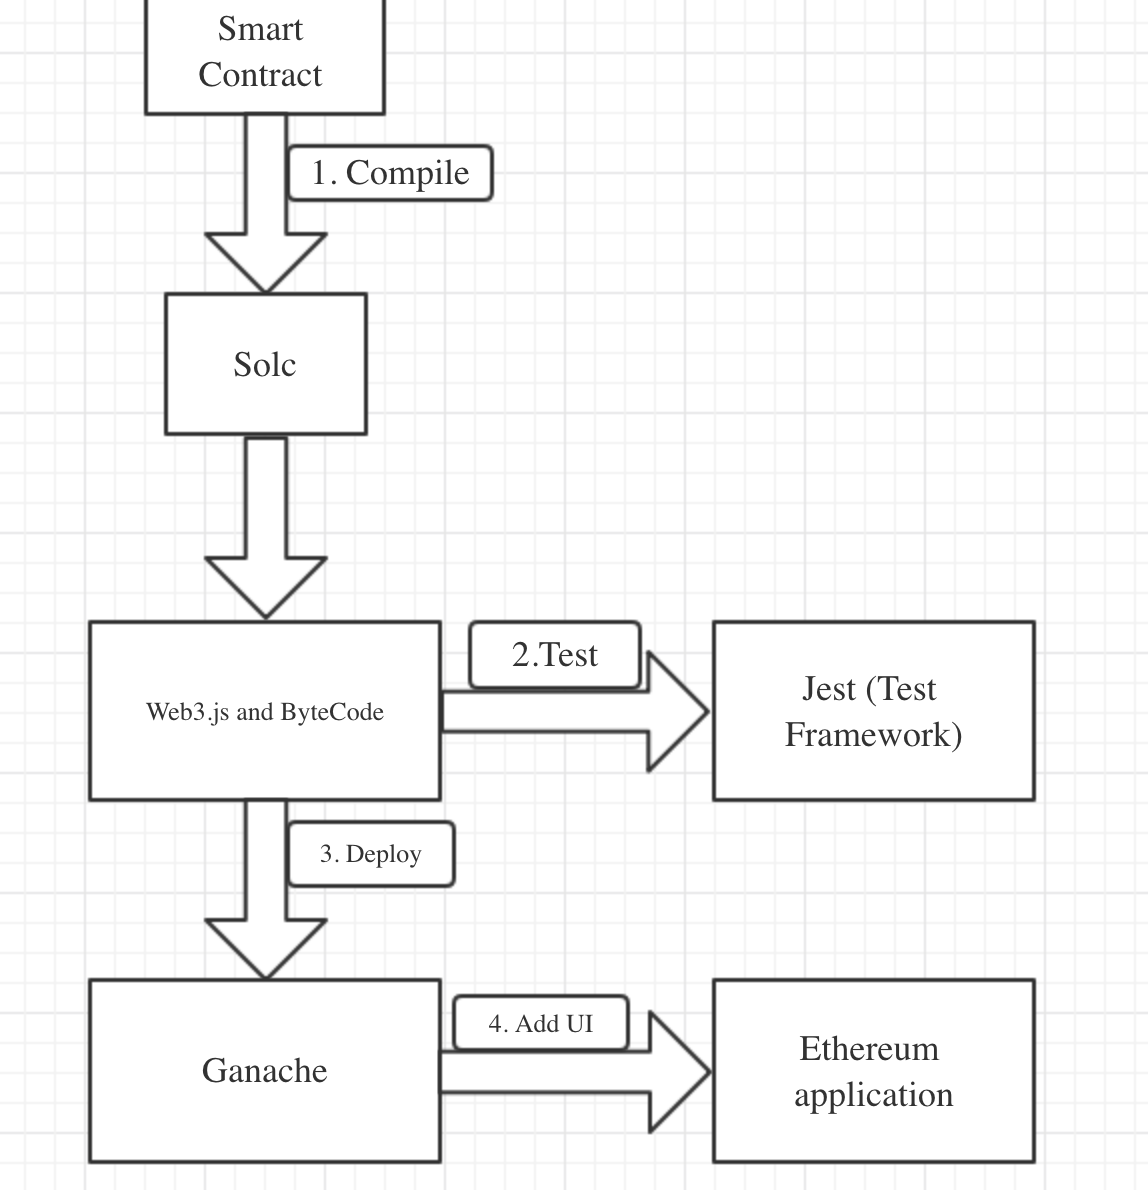
\includegraphics[width=0.8\textwidth]{developWorkFlow.png}
  \caption{Development workflow}
  \label{develop} 
\end{figure}
Inspiring by the truffle and remix, we could establish a basic workflow based on JavaScript ecosystem, which could be described as \ref{develop}.
After finishing the smart contract, Solc \cite{solc} which is Solidity compiler written in JavaScript will be used to compiled the source code.
Then web3.js and the compiled smart contracts will be used for tested by jest which is a JavaScript test framework. 
After passing all the test, the contracts will be deployed on the Ethereum test network by Ganache.
Then with the UI code, user will be able to use the application to do the academic publishing.
\section{Workspace setup}
Before starting write code, some prerequisites should be satisfied
\begin{itemize}
  \item \textbf{Git} Version control
  \item \textbf{Node.js} The major technology stack of the project is the JavaScript.
  \item \textbf{Npm} The nodejs package manager, which will help us to manage tools like Solc and Jest.
  \item \textbf{Text editor} It is suggested to use Vscode. 
\end{itemize}
After setting all the environment, a workspace should be initialed for the future development, 
which contains these directory:
\begin{itemize}
  \item \textbf{contracts} store the contracts source code
  \item \textbf{compiled} store the compiled contract
  \item \textbf{scripts} scripts used to start compile, test and deploy.
  \item \textbf{test} define how test will conducted. 
  \item \textbf{package.json} used for npm to manager the project.
\end{itemize}  
\section{The Paper contract}
\subsection{Source code}
\begin{lstlisting}[language=Solidity]
  pragma solidity ^0.4.24;
  contract SmartPaper is AuthorList{
    struct Version{
        uint versionNumber;
        bytes32 versionDescription;
        bytes32 metaData;
        bool isPublished;
        mapping (address => bool) signs;
        uint voterCount;
    }
    bytes32 private latestDescription;
    bytes32 private latestMetaData;
    bytes16 private latestPaper;
    uint public latestVersion;
    address private newAuthor; 
    uint private agreeCount;
    address[] public authors;
    mapping(address => bool) isAuthor;
    mapping(address => bool) isAgree;
    bytes16[] public md5List;
    Version[] public versions;
    mapping (bytes16 => Version) public versionMap;
    constructor (bytes32 _description, bytes32 _metaData, bytes16 _paperMD5, address[] _authors) public{
        require(_authors.length > 0, "Invalid authors list");
        authors = _authors;
        latestPaper = _paperMD5;
        md5List.push(latestPaper);
        latestMetaData = _metaData;
        latestDescription = _description;
        uint versionNumber = uint(1); 
        addAddressesToAuthorList(_authors);
        Version memory newVersion = Version({
            versionNumber: versionNumber,
            versionDescription:latestDescription,
            metaData:latestMetaData,
            isPublished:false,
            voterCount:1
        });
        versions.push(newVersion);
        versions[0].signs[msg.sender] = true;
        versionMap[latestPaper] = newVersion; 
        for(uint256 i = 0; i < _authors.length; i++){
            isAuthor[_authors[i]] = true;
            isAgree[_authors[i]] = false;
        }       
    }
    function checkIn() public onlyIfAuthor(msg.sender) payable{
        require(versions[0].signs[msg.sender] == false, "Ban");
        versions[0].signs[msg.sender] = true;
        versions[0].voterCount++;
        if(versions[0].voterCount == authors.length + 1){
            versions[0].isPublished = true;
            latestVersion = versions[0].versionNumber;
        }
        versionMap[md5List[0]] = versions[0];
    }
    function createNewVersion(bytes32 versionDescription, bytes32 metaData, bytes16 md5) public
    onlyIfAuthor(msg.sender) payable {
        uint versionNumber = latestVersion + 1;
        Version memory newVersion = Version({
            versionNumber: versionNumber,
            versionDescription:versionDescription,
            metaData:metaData,
            isPublished:false,
            voterCount:1
        });
        md5List.push(md5);
        versions.push(newVersion);
        versionMap[md5] = newVersion;
    }
    function addNewAuthor(address _newAuthor) public onlyIfAuthor(msg.sender) payable{
        require(newAuthor==address(0), "Ban");
        newAuthor = _newAuthor;
        agreeCount = 0;
    }
    function approveNew(address _newAuthor) public onlyIfAuthor(msg.sender) payable{
        require(newAuthor == _newAuthor,"BAN");
        agreeCount++;
        isAgree[msg.sender] = true;
        if(agreeCount == authors.length){
            addAddressToAuthor(newAuthor);
            authors.push(newAuthor);
            isAuthor[newAuthor] = true;
            newAuthor = address(0);
            agreeCount = 0;
            for(uint i = 0; i<authors.length; i++){
                isAgree[authors[i]] = false;
            }
        }
    }
    function approveVersion(uint _versionNumber, bytes16 md5)  public onlyIfAuthor(msg.sender) payable{
        Version storage version = versions[_versionNumber-1];
        require(!version.signs[msg.sender], "BAN");
        version.signs[msg.sender] = true;
        version.voterCount++;
        if(version.voterCount==authors.length + 1){
            version.isPublished = true;
            latestVersion = version.versionNumber;
            latestDescription = version.versionDescription;
            latestMetaData = version.metaData;
            latestPaper = md5;
            versionMap[md5] = version;
            require(versionMap[md5].versionNumber == versions[_versionNumber-1].versionNumber, "BAN");
            require(versionMap[md5].versionDescription == versions[_versionNumber-1].versionDescription, "BAN");
            require(versionMap[md5].isPublished == versions[_versionNumber-1].isPublished, "BAN");
            require(versionMap[md5].metaData == versions[_versionNumber-1].metaData, "BAN");
            require(versionMap[md5].voterCount == versions[_versionNumber-1].voterCount, "BAN");
            require(latestVersion == versions[_versionNumber-1].versionNumber, "BAN");
        }
        versionMap[md5] = version;
    }
} 
\end{lstlisting}
It could be noticed that the implementation of Paper contract is more complicated than the design. 
There are some extra private properties to help contract to manage the internal state. 
It has six major public application interface which is design to satisfy the requirements.
One of the authors firstly create a paper by using the \textbf{createNewPaper(constructor)}, 
then the other author need to use \textbf{checkIn} to approve the initial version.
If a new version need to be published, an author will use \textbf{createNewVersion}. 
All the other authors need to user \textbf{approveVersion} to make sure they have the consensus.
If the team decide to add a new number, they could do that by \textbf{addNewAuthor} and \textbf{approveNewAuthor}.
Every time the user want to use these function, 
it will start a transaction on the Ethereum which means they need to pay for it.
The transaction will be handled by a Ethereum wallet. It is typically a browser extension. 
A popular example would be MetaMask \cite{metamask}. 
It is vital to remind of users to download the extension to use the application.
These contract also provides user with many useful tools which is free. 
\textbf{isAuthor} is an example that can quickly check if an user belongs to this paper.
\section{Compile, Test, Deploy}
\subsection{Compile}
Since the smart contract has finished, the next step would be compile these contracts by Solc.
\begin{figure}[H]
  \centering
  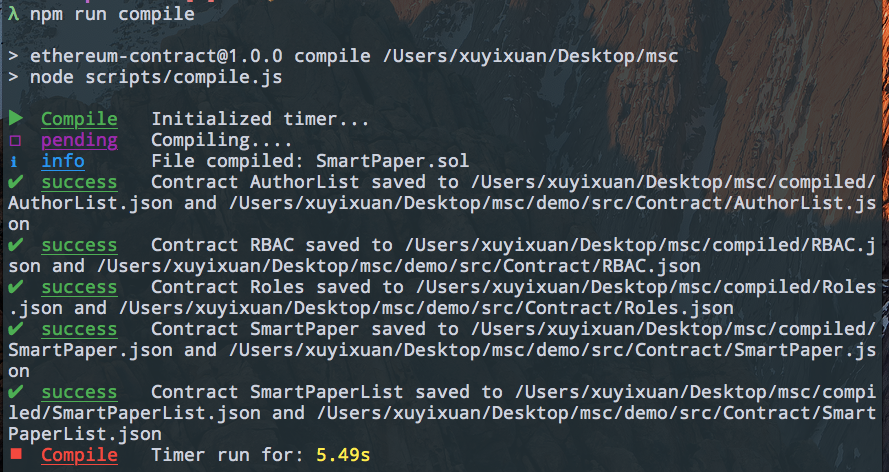
\includegraphics[width=0.8\textwidth]{compile.png}
  \caption{Compile Result}
  \label{compile} 
\end{figure}
All the contracts will be complied into JSON format so that developer could easily use JavaScript to use these contracts to interact with the Ethereum network.
There are some internal contracts also being compiled but developers do not need to care about them. The two key contracts are \textbf{SmartPaper} and \textbf{SmartPaperList}.
The SmartPaperList contract is used to manage all the smartPaper. 
It stores all the addresses of the smartPaper so that user dont have to remember all addresses they created.
It could also help the client side to implements the functionality of searching.
\subsection{Test}
The next step for development flow is testing.
\begin{figure}[H]
  \centering
  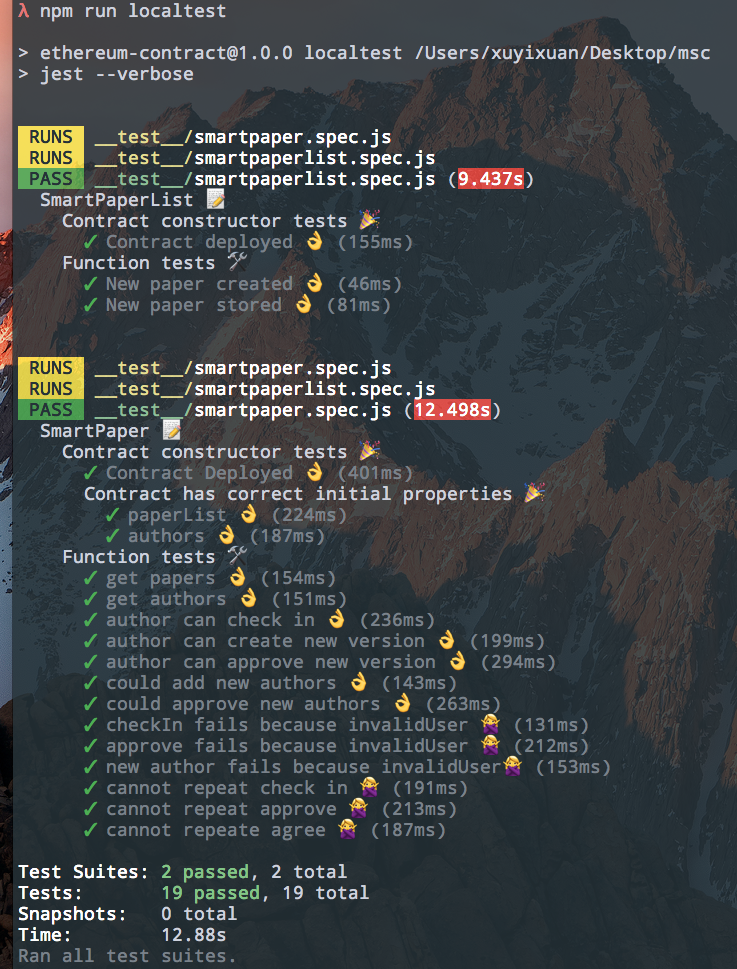
\includegraphics[width=0.8\textwidth]{test.png}
  \caption{Test Result}
  \label{test} 
\end{figure}
Testing is really implement for the robustness of software. 
JavaScript ecosystem has lots of useful tools to help us do the.
Jest, which is a JavaScript test framework, 
provides us with useful information about the result of tests in the terminal.
There are 19 unit tests for those two key contracts which means all the functionalities are tested. Although tests cannot eliminate bugs,
those tests could give a strong fundamental base to iterate the development of contracts. Every time the contracts code changes, 
all the test will be re-run to make sure the changes won't break the previous code. 
New test should be added if there are new functionalities.
\subsection{Deploy}
The last step for development flow is deploying. 
The contracts have be deployed on the Ethereum network to become a public service.
\begin{figure}[H]
  \centering
  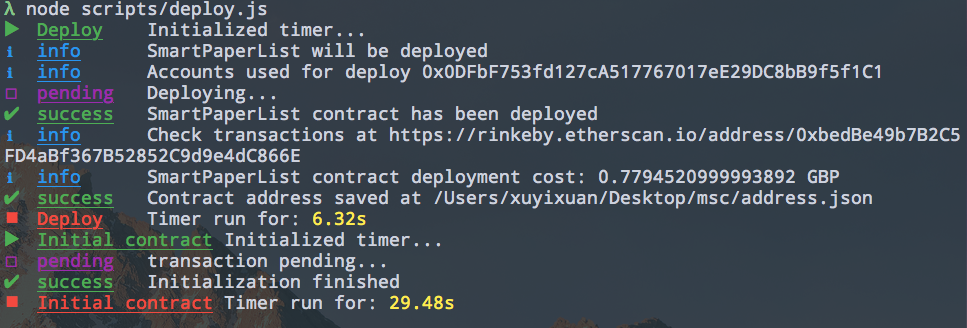
\includegraphics[width=0.9\textwidth]{deploy.png}
  \caption{Deploy Result}
  \label{deploy} 
\end{figure}
A smartPaperList contract will be deployed, which is the entry point of the application.
The contract will be used to keep track of 
all the smart papers created under this contract 
so that user does not need to remember every addresses of their smart papers. 
The development process is also a transaction. 
In \ref{deploy}, the hash of transaction is displayed for developer to check. 
Once a transaction is finished, 
the address of smartPaperList contract will be returned and stored on disk. 
The address will be used for the application development. 
The authors will use this address to use smartPaperList to create smart paper instead of directly creating the smart paper.
It is more convenient for authors to manage their papers.
\subsection{Continues Integration}
Since the workflow has been established, we would like to automate the whole process rather than running them by head.
In this project, the GitLab CI is used for continue integration. 
Once a new version is pushed onto GitLab, 
it will have a pipeline that run the three steps of development workflow.
Once all the steps is successful, the continues integration will pass. 
This could really help to have a better robustness of our project.
\begin{figure}[H]
  \centering
  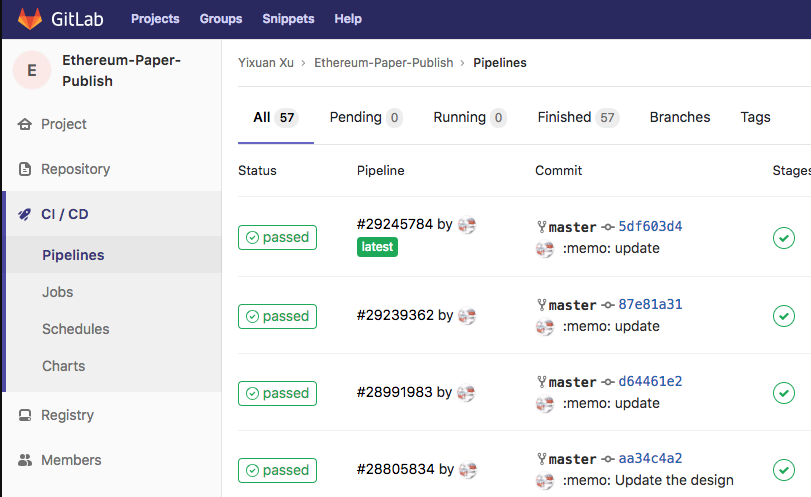
\includegraphics[width=0.9\textwidth]{ci.png}
  \caption{Continues Integration Result}
  \label{ci} 
\end{figure}
\section{Client development}
The user of the client would be authors and reviewers. 
Author will create papers, approve papers, create versions and approve versions. 
For a Ethereum application, there is no need for user system. 
Authors and reviewers just need to use their accounts of the Ethereum. 
However, the application do need a Ethereum wallet. Users have to download a Ethereum wallet in advance,
which is the only part that is different from the current web service.
We chose the MetaMask which is a really user-friendly Ethereum wallet for the client.
For a typical web application, the flow of the information would be list -- details -- interact. 
In the application, it would be:
\begin{itemize}
  \item List of paper -- details of a specific paper -- Add new paper
  \item Details of a specific paper -- list of versions -- Add new version or new author
\end{itemize}
So that we need three forms to help the authors to submit their jobs.
\begin{itemize}
  \item \textbf{The new paper form} this form will be used for authors to create a new paper. the address of new paper will be stored in paper list
  \item \textbf{The new version form} this form will be used for authors to create a new version. The paper will have a list of version.
  \item \textbf{The new author form} this form will be used for authors to add a new author.
\end{itemize}
The client is a modern JavaScript single page application implemented by React.js \cite{react}.
The source code could be found at \href{https://gitlab.com/yixuanxu94/Ethereum-Paper-Publish}{Ethereum-Paper-Publish}.
\begin{figure}[H]
  \centering
  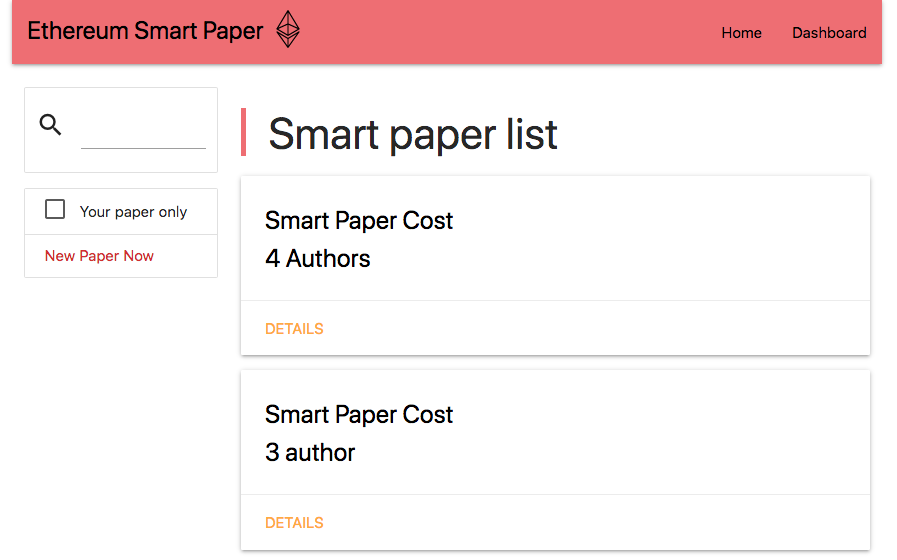
\includegraphics[width=0.9\textwidth]{app1.png}
  \caption{List of smart paper}
  \label{list} 
\end{figure}
\begin{figure}[H]
  \centering
  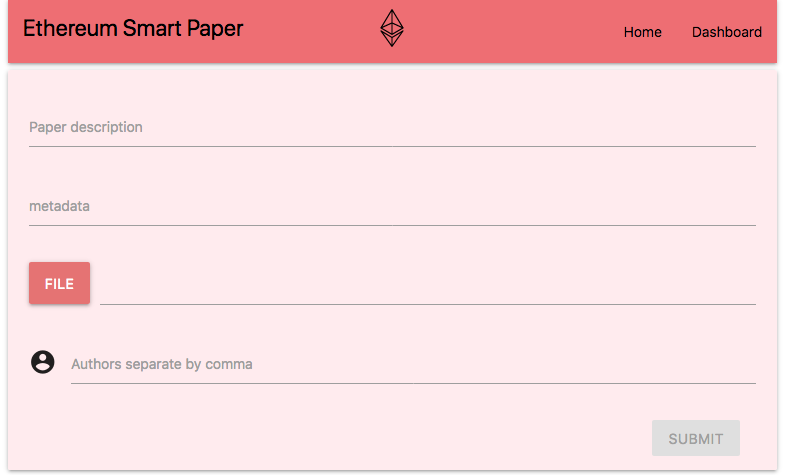
\includegraphics[width=0.9\textwidth]{app2.png}
  \caption{The new paper form}
  \label{form}
\end{figure}
\chapter{Evaluation}
The aim of the project is to do the cost analysis of the application implemented in chapter 4.
This would be the key index for the evaluation of the project.
\section{Cost analysis}
\subsection{Ecosystem in ethereum}
Before doing the cost analysis, the first step is to understand the ecosystem in the ethereum.
\subsubsection{Gas}
Each low level operations available in the Ethereum network is called OPCODE. It contains some operations such as ADD, CREATE.
Those OPCODEs comes with a number called 'gas'. Gas is an abstract number that represented the complexity of the current operation.
Typically, ADD will use three gas and MUL will use five gas, it could be noticed that MUL is more complex than ADD. What's more, 
all the transactions will cost 210000 gas as a base.
\subsubsection{Gas price}
Gas is fixed per operation, but the price of gas is dynamic and is determined by the market. 
Gas price is the value that represents how much Ether the user is going to pay per user. When users send transactions, they will be asked to set a gas price.
The miners will be paid out this fee, so the transactions with higher gas price will be recorded with higher priority. The actual cost would be:
\begin{equation}
  totalCost = gasPrice * gasUsed
\end{equation}
\subsubsection{Gas limit}
Gas limit refers to the maximum amount of gas that can be used for a single transaction.
More computational work need higher gas limit. For our analysis, we using the default gas limit which is 2100000 gas.
Gas limit is a special mechanism to prevent user from spending two much Ether due to buggy codes or errors on the Ethereum network. 
\subsection{Result}
In project, the cost of creating a new paper and releasing a new version are the two major index that matters.
After doing some experiment, it is found out that the key factor which would affect the cost is the number of authors.
After using the automate testing scripts to collect the data, the result is visualized.
\subsubsection{The cost of creating a new paper}
\begin{figure}[H]
  \centering
  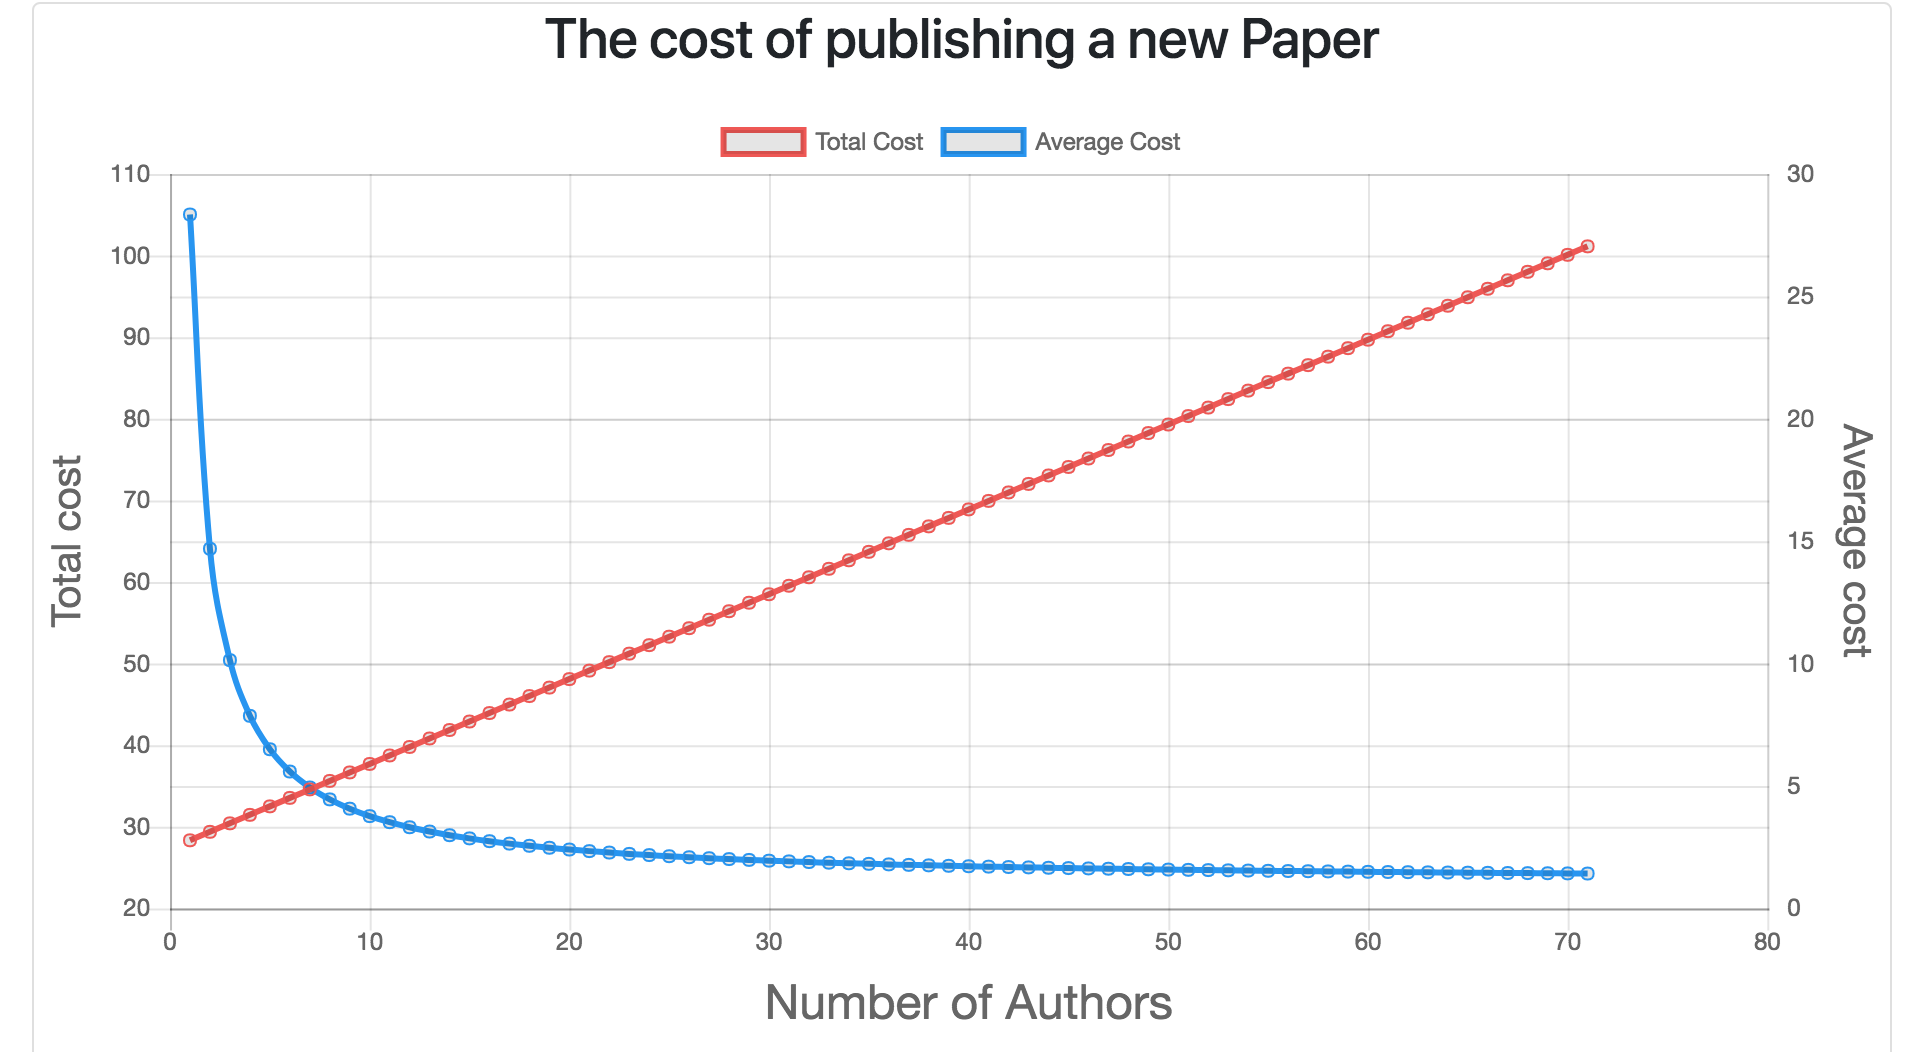
\includegraphics[width=1\textwidth]{papercost.png}
  \caption{The cost of creating a new version}
  \label{papercost}
\end{figure}
\chapter{Discussion}
\section{Good}
\section{Bad}
\chapter{Conclusion}
\backmatter
\bibliographystyle{ieee}
\bibliography{ECS}
\end{document}
%% ----------------------------------------------------------------
